\documentclass{article}
\usepackage{graphicx}
\usepackage{hyperref}
\usepackage{tikz}
\usepackage{float}
\usepackage{verbatim} % Ya viene en LaTeX por defecto
\usepackage[a4paper, top=1.5cm, bottom=2.5cm, left=2.5cm, right=2.5cm]{geometry}
\usepackage{listings}
\usepackage{xcolor} % opcional para colores
\setlength{\parindent}{0pt}
\setlength{\parskip}{0.5em}   % Espacio entre p\'arrafos
\usetikzlibrary{arrows.meta, positioning}

\begin{document}
\begin{titlepage}
    \begin{center}
        
\includegraphics[width=0.2\textwidth]{unam.png}
        \vspace*{.5cm}

        \LARGE
        \textbf{Universidad Nacional Aut\'onoma de M\'exico}

        \vspace{0.5cm}
        \LARGE
        Facultad de Estudios Superiores Acatl\'an


        \vspace{2cm}

        \textbf{Programaci\'on de paralela y concurrente} \\
        \vspace{0.5cm}
        \textbf{Practica 1} \\
        Simulaci\'on de un sistema de Hospitalario \\


        \vfill

        \vspace{1cm}

        \textbf{\large Autor:} \\
        Jorge Miguel Alvarado Reyes \\
        \textbf{\large No. Cuenta:} \\
        421010301\\
        \vspace{.5cm}
        \normalsize \today

    \end{center}
\end{titlepage}

\tableofcontents

\newpage

\section*{Objetivo}
El objetivo de esta práctica es aplicar los paradigmas de programación paralela, concurrente y asincrónica mediante la simulación de un sistema hospitalario que imita el flujo real de atención médica en urgencias.

\section{Diseño del flujo hospitalario}

Antes de comenzar con la implementación del código, fue necesario realizar un recorrido mental del proceso de atención en urgencias, identificando los pasos clave que sigue un paciente desde su llegada al hospital hasta su egreso. Este análisis permitió establecer un flujo lógico que se representa en el siguiente diagrama:

\begin{figure}[H]
    \centering
    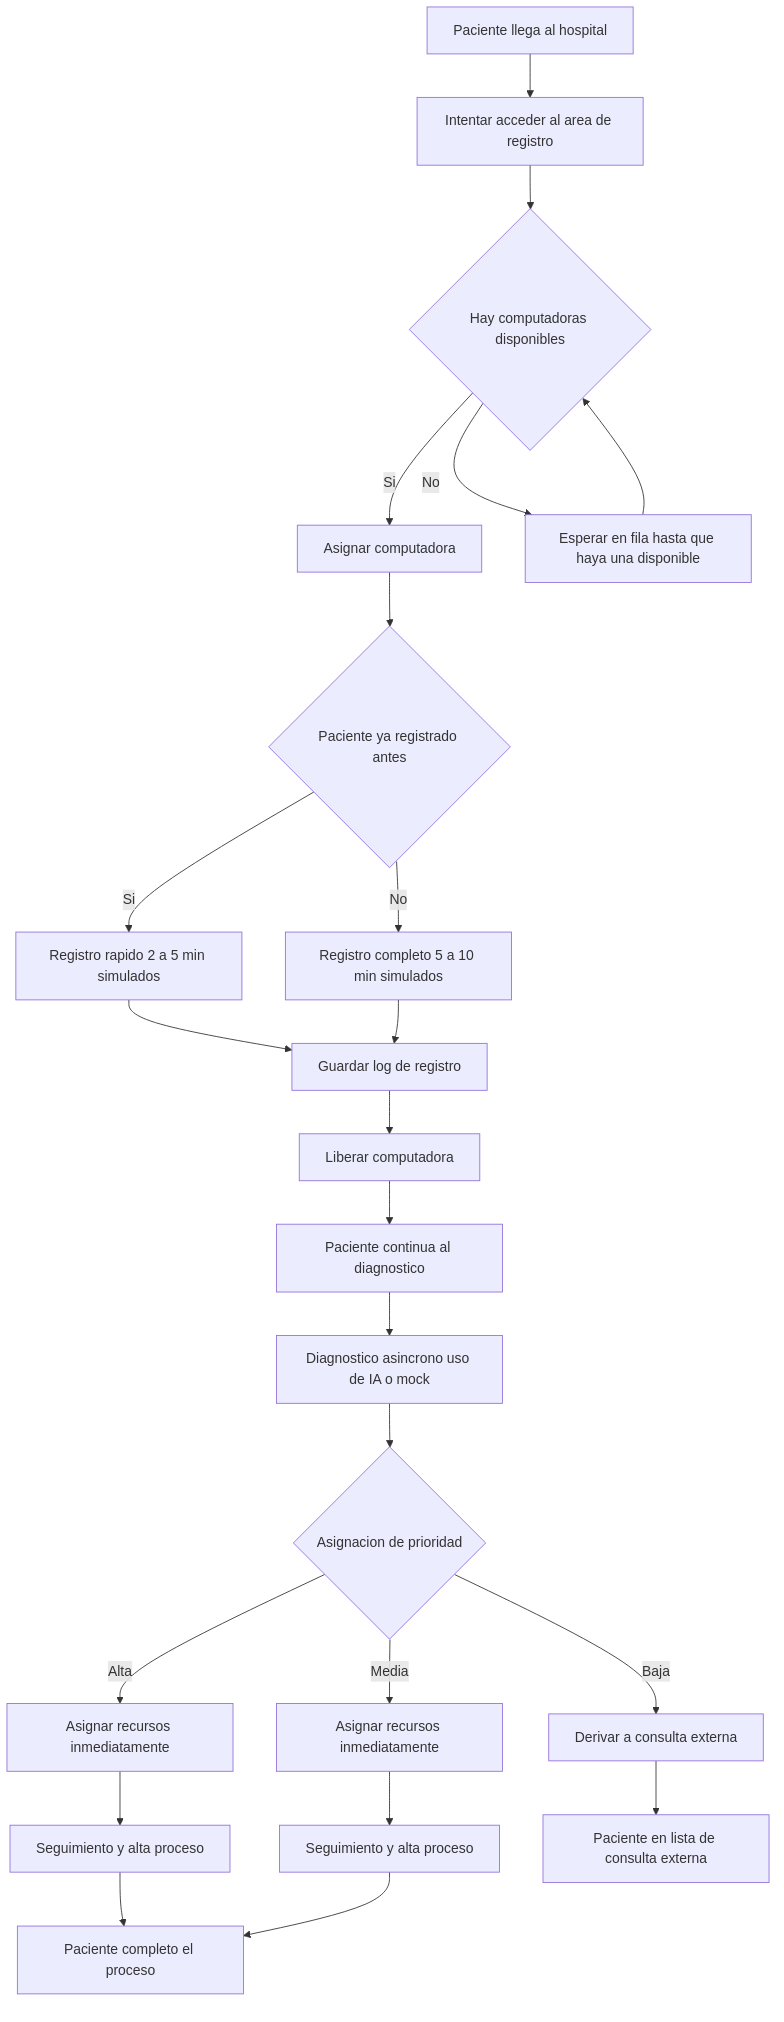
\includegraphics[width=0.4\textwidth]{flujo_hospital.png}
    \caption{Diagrama de flujo del sistema hospitalario simulado}
\end{figure}

\newpage

\subsection{Estructura de un paciente}

Cada paciente en la simulación es representado mediante una estructura que contiene la siguiente información:

\begin{itemize}
    \item \textbf{ID:} Identificador único generado automáticamente.
    \item \textbf{Nombre:} Nombre del paciente.
    \item \textbf{Género:} Masculino, femenino u otro.
    \item \textbf{Edad:} Edad en años.
    \item \textbf{Raza:} Característica demográfica relevante para el diagnóstico.
    \item \textbf{Altura:} Estatura del paciente en metros.
    \item \textbf{Peso:} Peso del paciente en kilogramos.
    \item \textbf{Hábitos alimenticios:} Descripción general de su alimentación.
    \item \textbf{Antecedentes médicos:} Lista de condiciones médicas previas o enfermedades crónicas.
    \item \textbf{Registrado:} Indica si el paciente ya había sido registrado anteriormente en el sistema.
    \item \textbf{Síntomas:} Cadena de texto que describe lo que el paciente está sintiendo o experimentando al llegar al hospital (por ejemplo: "dolor de cabeza, fiebre y tos leve").
\end{itemize}

Esta estructura permite simular de forma realista distintos perfiles de pacientes y es utilizada a lo largo de todo el flujo hospitalario: registro, diagnóstico, asignación de recursos y alta.


\section{Estructura del sistema}

\subsection{Organización modular del código}

Se decidió separar la lógica de cada componente del sistema en módulos independientes, siguiendo el principio de responsabilidad única, donde cada módulo cumple una función específica.

La estructura general del sistema es la siguiente:

\begin{verbatim}
    hospital/
    +-- .venv/                     # Entorno virtual de Python
    +-- data/                      
    |   +-- paciente.py           # Clase Paciente (estructura de persona real) 
    |   +-- pacientes.py          # Conjunto de pacientes
    +-- diagnostico_ia.py         # Funcion de diagnostico con OpenIA
    +-- diagnostico_mock.py       # Diagnóstico simulado para pruebas
    +-- logger_datos.py           # Registro de eventos en archivos CSV
    +-- main.py                   # Ejecuta el flujo de la simulación
    +-- recursos.py               # Asignación de camas, doctores, etc.
    +-- registro.py               # Flujo de registro de un paciente
    +-- seguimiento.py            # Seguimiento y alta de pacientes
\end{verbatim}

\section{Implementación técnica}

\subsection{Uso de librerías}

Para llevar a cabo la simulación del sistema hospitalario, se emplearon diversas librerías estándar de Python que permiten gestionar la concurrencia, el paralelismo y la asincronía, así como medir tiempos y manejar estructuras de datos compartidas:

\begin{itemize}
    \item \texttt{time} — Utilizada para manejar los tiempos simulados dentro del sistema.
    \item \texttt{random} — Empleada para simular variabilidad en los tiempos de espera y decisiones dentro del flujo.
    \item \texttt{threading} — Permite la ejecución concurrente de múltiples pacientes simulados mediante hilos.
    \item \texttt{asyncio} — Utilizada para operaciones asincrónicas, como simulaciones de diagnósticos realizados por IA o APIs externas.
    \item \texttt{multiprocessing} — Empleada para ejecutar tareas en paralelo, como el procesamiento intensivo de diagnósticos en múltiples núcleos.
    \item \texttt{datetime} — Para registrar con precisión eventos temporales en los logs.
    \item \texttt{queue} — Utilizada para coordinar el acceso a recursos limitados (como computadoras de registro o camas).
\end{itemize}

\subsection{Simulación del flujo hospitalario: \texttt{main.py}}

El archivo \texttt{main.py} orquesta el flujo completo del sistema hospitalario. Cada paciente es procesado en un hilo independiente, simulando concurrencia real en un entorno hospitalario. A continuación se describe el flujo general implementado:

\begin{itemize}
    \item Se define un modo de diagnóstico (\texttt{"mock"} o \texttt{"ia"}) que determina si se usa un diagnóstico simulado o uno basado en IA.
    \item Se crea una cola prioritaria para organizar a los pacientes según su nivel de urgencia.
    \item La función \texttt{flujo\_paciente} representa el recorrido de un paciente a través del sistema:
          \begin{itemize}
              \item Registro del paciente (bloque concurrente con \texttt{threading}).
              \item Diagnóstico asincrónico usando \texttt{asyncio}.
              \item En caso de prioridad \texttt{Alta} o \texttt{Media}, se asignan recursos y se realiza el seguimiento del paciente en un proceso separado (\texttt{multiprocessing}).
              \item Para prioridad \texttt{Baja}, el paciente es derivado a consulta externa.
          \end{itemize}
    \item El archivo principal inicia hilos para cada paciente y espera a que todos terminen antes de finalizar la simulación.
\end{itemize}

\subsection{Registro concurrente de pacientes: \texttt{registro.py}}

La función \texttt{registrar\_paciente} simula la llegada y registro de un paciente en el sistema. Para este propósito, se utiliza un \texttt{BoundedSemaphore} que limita el acceso simultáneo a un máximo de 5 pacientes, representando cinco computadoras disponibles.

Además, se utiliza una \texttt{Queue} compartida para asignar dinámicamente el identificador de la computadora disponible. Este enfoque permite una gestión realista de recursos compartidos.

Durante el registro, se simula el tiempo de espera y el tiempo de atención, diferenciando entre registros rápidos (pacientes recurrentes) y registros completos (pacientes nuevos). Al finalizar, se guarda un log con los datos del evento.

\subsection{Diagnóstico asincrónico simulado: \texttt{diagnostico\_mock.py}}

El módulo \texttt{diagnostico\_mock.py} representa el diagnóstico médico realizado a cada paciente. Esta etapa fue diseñada como una función \texttt{async} para simular llamadas a una API de inteligencia artificial con latencia variable. Utiliza la librería \texttt{asyncio} para suspender la ejecución durante un tiempo aleatorio que representa la duración del análisis médico (entre 5 y 10 minutos simulados).

La función genera un diagnóstico aleatorio entre varias opciones posibles y clasifica la prioridad del paciente de acuerdo con el contenido del texto. Esta prioridad se utiliza más adelante para decidir si el paciente debe recibir atención inmediata o ser derivado a consulta externa.

También se registra el diagnóstico en un archivo CSV mediante la función \texttt{guardar\_log()}.

\subsection{Diagnóstico con Inteligencia Artificial (OpenAI)}

Además del diagnóstico simulado, se implementó una variante que utiliza la API de OpenAI para generar un diagnóstico preliminar con base en las características del paciente. Esta opción representa un escenario más realista donde se consulta un modelo de lenguaje entrenado con información médica general.

Para la integración se empleó el cliente \texttt{AsyncOpenAI} del SDK oficial de OpenAI (\texttt{openai >= 1.0.0}), el cual permite realizar llamadas asincrónicas a modelos como \texttt{gpt-3.5-turbo}. El flujo del diagnóstico IA se adapta de forma dinámica a los datos del paciente, incluyendo síntomas, antecedentes médicos y características demográficas.

El modelo retorna un diagnóstico estructurado en tres secciones:
\begin{itemize}
    \item \textbf{Diagnóstico:} Hipótesis clínica redactada en lenguaje técnico.
    \item \textbf{Prioridad:} Nivel de atención sugerido (\texttt{Alta}, \texttt{Media} o \texttt{Baja}).
    \item \textbf{Recomendación:} Acciones médicas sugeridas para el caso.
\end{itemize}

El siguiente fragmento muestra un ejemplo del mensaje enviado al modelo:

\begin{quote}
\texttt{Eres un médico de urgencias en un hospital. Realiza un diagnóstico preliminar con base en los siguientes datos del paciente: [...] Proporciona un diagnóstico clínico inicial en lenguaje técnico y profesional. Incluye una prioridad de atención y una recomendación.}
\end{quote}

Esta variante es controlada mediante la variable \texttt{MODO\_DIAGNOSTICO} que permite cambiar entre \texttt{mock} e \texttt{ia}.

Se eligió la variante asincrónica ya que este tipo de operación puede tener latencia considerable. De este modo se evita bloquear la ejecución del resto del sistema hospitalario mientras se espera la respuesta del modelo.

\subsection{Asignación de recursos hospitalarios}

Una vez que un paciente recibe prioridad \texttt{Alta} o \texttt{Media}, es dirigido al área médica para ser atendido. En esta fase se modela la disponibilidad limitada de recursos mediante semáforos que controlan el acceso a camas y doctores:

\begin{itemize}
    \item \textbf{Camas disponibles:} Se limita el acceso a un máximo de 10 pacientes simultáneamente mediante un semáforo.
    \item \textbf{Doctores disponibles:} Solo hay 5 doctores disponibles para consulta en paralelo.
\end{itemize}

El flujo general de esta etapa es el siguiente:

\begin{enumerate}
    \item El paciente espera una cama disponible. Al obtenerla, permanece en observación un tiempo aleatorio (simulado entre 15 y 30 minutos reales).
    \item Posteriormente, espera a ser atendido por un doctor. La consulta médica tiene una duración simulada de entre 20 y 40 minutos.
    \item Al finalizar la atención, el paciente libera los recursos y se registra un log detallado con los tiempos de espera y duración de cada fase.
\end{enumerate}

\newpage

\section*{Demostración de ejecución}

A continuación se muestra un ejemplo real del flujo completo que sigue un paciente dentro del sistema hospitalario. Este registro corresponde al caso de \textbf{Lucía Martínez}, quien fue atendida con prioridad alta debido a una crisis asmática.

\begin{verbatim}
[IngresoHospital][12:31:13] - Lucía Martínez ha ingresado al sistema.

[RegistroLlegada][12:31:13] 
- Lucía Martínez llegó al área de registro y está esperando computadora...
[RegistroComienzo][12:31:13] - Lucía Martínez comenzó su registro en computadora 1 (esperó 0.00 s).
[RegistroFin] - Lucía Martínez terminó su registro (completo (nuevo)) en 0.54 s en computadora 1.

[12:31:13] Lucía Martínez está en diagnóstico (OpenAI)...
[IA] Diagnóstico para Lucía Martínez (12:31:15):
Diagnóstico: Crisis asmática aguda
Prioridad: Alta
Recomendación: 
Administer broncodilatadores de acción rápida como salbutamol, oxigenoterapia
y evaluar la necesidad de corticosteroides sistémicos. Realizar monitoreo
continuo de la saturación de oxígeno y la función respiratoria. 
Considerar hospitalización si no hay mejoría significativa.

[DiagnósticoListo] Lucía Martínez encolado con prioridad Alta
[Asignación] Lucía Martínez en atención inmediata.

[EsperaCama] - Lucía Martínez esperando cama...
[AsignacionCama][12:31:15] - Lucía Martínez fue asignado a una cama (esperó 0.00 s).
[EsperaDoctor] - Lucía Martínez esperando doctor...
[ConsultaInicio][12:31:17] - Lucía Martínez atendido por un doctor (esperó 0.00 s).
[ConsultaFin][12:31:20] - Lucía Martínez terminó su consulta.
[SalidaAreaMedica] - Lucía Martínez liberó cama y salió del área médica.

[ObservacionInicio][12:31:20] - Lucía Martínez está en observación post-consulta...
[Alta][12:31:23] - Lucía Martínez ha sido dado de alta tras 3.43 segundos de observación.

Lucía Martínez ha completado su proceso.

[Main] Todos los pacientes han sido atendidos o derivados a consulta externa.
\end{verbatim}

Este ejemplo ilustra de forma detallada cómo se registran los eventos en tiempo real, permitiendo validar el comportamiento del sistema y analizar su desempeño bajo condiciones de concurrencia y procesamiento asincrónico.


\end{document}